\documentclass[10pt,compress,usetitleprogressbar,mathserif]{beamer}
\usepackage[spanish, es-tabla,es-noquoting,es-noshorthands]{babel}
\usepackage{tikz}
\usepackage{showexpl}
\usepackage{amsthm}
\usepackage{amsmath}
\usepackage{amssymb}
\usepackage{graphicx}
\usepackage{adjustbox} % Tamaño de tablas
\graphicspath{{img/}}
\usepackage{booktabs}% http://ctan.org/pkg/booktabs
% Solarized palette
\definecolor{solarizedBase03}{HTML}{002B36}
\definecolor{solarizedBase02}{HTML}{073642}
\definecolor{solarizedBase01}{HTML}{586e75}
\definecolor{solarizedBase00}{HTML}{657b83}
\definecolor{solarizedBase0}{HTML}{839496}
\definecolor{solarizedBase1}{HTML}{93a1a1}
\definecolor{solarizedBase2}{HTML}{EEE8D5}
\definecolor{solarizedBase3}{HTML}{FDF6E3}
\definecolor{solarizedYellow}{HTML}{B58900}
\definecolor{solarizedOrange}{HTML}{CB4B16}
\definecolor{solarizedRed}{HTML}{DC322F}
\definecolor{solarizedMagenta}{HTML}{D33682}
\definecolor{solarizedViolet}{HTML}{6C71C4}
\definecolor{solarizedBlue}{HTML}{268BD2}
\definecolor{solarizedCyan}{HTML}{2AA198}
\definecolor{solarizedGreen}{HTML}{859900}

\setbeamercovered{dynamic}

\usetheme{epstfg}
\setbeamertemplate{note page}[compress]
\title{Práctica 1}
\author{Pablo Baeyens \and Antonio Checa \and Iñaki Madinabeitia \and José Manuel Muñoz \and Darío Sierra}
\date{Algorítmica}
\def\inline{\lstinline[basicstyle=\ttfamily]}

\begin{document}
\maketitle

\begin{frame}{Índice}
  \tableofcontents
\end{frame}

\section{Ejercicio 1: \large{Eficiencia Empírica }}

\subsection{Algoritmos Cuadráticos}

\begin{frame}{Burbuja}
	\resizebox{\linewidth}{!}{
		\hspace{1cm}
		\begin{tabular}{|l|l|l|l|l|l|}
	\hline
	Tamaño & Antonio & Darío & Iñaki & José Manuel & Pablo \\
	\hline
	\hline
	2000 & 0,011413 & 0,0146897 & 0,0140894 & 0,00961352 & 0,00950047 \\
	\hline
	10000 & 0,285049 & 0,292014 & 0,317834 & 0,319125 & 0,256134 \\
	\hline
	18000 & 0,9231 & 0,957501 & 1,05149 & 1,12075 & 0,893985 \\
	\hline
	26000 & 1,93603 & 2,30372 & 2,1866 & 2,41593 & 1,91995 \\
	\hline
	34000 & 3,31074 & 3,46101 & 3,72809 & 4,20884 & 3,42199 \\
	\hline
	42000 & 5,26566 & 5,59224 & 5,69877 & 6,46732 & 5,13279 \\
	\hline
	50000 & 8,1269 & 7,95426 & 8,08572 & 9,2569 & 7,48556 \\
	\hline
\end{tabular}

	}
\end{frame}

\begin{frame}{Selección}
	\resizebox{\linewidth}{!}{
		\hspace{1cm}
		\begin{tabular}{|l|l|l|l|l|l|}
	\hline
	Tamaño & Antonio & Darío & Iñaki & José Manuel & Pablo \\
	\hline
	\hline
	2000 & 0,00515467 & 0,0188928 & 0,0056981 & 0,00642196 & 0,0100637 \\
	\hline
	10000 & 0,121217 & 0,121786 & 0,133457 & 0,158756 & 0,126158 \\
	\hline
	18000 & 0,410265 & 0,393202 & 0,436515 & 0,515545 & 0,409696 \\
	\hline
	26000 & 0,872412 & 0,817823 & 0,902801 & 1,07721 & 0,853734 \\
	\hline
	34000 & 1,50895 & 1,62408 & 1,5385 & 1,84905 & 1,46012 \\
	\hline
	42000 & 2,35229 & 2,29655 & 2,34051 & 2,81587 & 2,22564 \\
	\hline
	50000 & 3,40647 & 3,47501 & 3,3125 & 3,98744 & 3,15386 \\
	\hline
\end{tabular}

	}

\end{frame}

\begin{frame}{Inserción}
	\resizebox{\linewidth}{!}{
		\hspace{1cm}
		\begin{tabular}{|l|l|l|l|l|l|}
	\hline
	Tamaño & Antonio & Darío & Iñaki & José Manuel & Pablo \\
	\hline
	\hline
	2000 & 0,0044917 & 0,00745713 & 0,00500529 & 0,00545271 & 0,0136858 \\
	\hline
	10000 & 0,107932 & 0,107475 & 0,119386 & 0,139938 & 0,106441 \\
	\hline
	18000 & 0,368311 & 0,345483 & 0,394836 & 0,43881 & 0,344915 \\
	\hline
	26000 & 0,760331 & 0,903855 & 0,816444 & 0,903978 & 0,711269 \\
	\hline
	34000 & 1,33726 & 1,76733 & 1,35952 & 1,53781 & 1,21549 \\
	\hline
	42000 & 2,08887 & 2,29417 & 2,09879 & 2,34337 & 1,84894 \\
	\hline
	50000 & 3,02904 & 3,52064 & 2,92835 & 3,32697 & 2,62017 \\
	\hline
\end{tabular}

	}
\end{frame}

\subsection{Algoritmos Cúbicos}

\begin{frame}{Algoritmo de Floyd}
	\resizebox{\linewidth}{!}{
		\hspace{1cm}
		\begin{tabular}{|l|l|l|l|l|l|}
	\hline
	Tamaño & Antonio & Darío & Iñaki & José Manuel & Pablo \\
	\hline
	\hline
	30 & 0,000224592 & 0,000625181 & 0,000280424 & 0,000377972 & 0,000661632 \\
	\hline
	150 & 0,0186866 & 0,0403935 & 0,0211072 & 0,024806 & 0,0200893 \\
	\hline
	270 & 0,104221 & 0,106563 & 0,119058 & 0,141979 & 0,110954 \\
	\hline
	390 & 0,314773 & 0,390241 & 0,358154 & 0,445757 & 0,328791 \\
	\hline
	510 & 0,692464 & 0,847743 & 0,790683 & 0,965839 & 0,735368 \\
	\hline
	630 & 1,30571 & 1,40966 & 1,47915 & 1,82847 & 1,37284 \\
	\hline
	750 & 2,27876 & 2,69492 & 2,48584 & 3,03609 & 2,3061 \\
	\hline
\end{tabular}

	}
\end{frame}

\subsection{Algoritmos $n\cdot log(n)$ }

\begin{frame}{Quicksort}
	\resizebox{\linewidth}{!}{
		\hspace{1cm}
		\begin{tabular}{|l|l|l|l|l|l|}
	\hline
	Tamaño & Antonio & Darío & Iñaki & José Manuel & Pablo \\
	\hline
	\hline
	1000000 & 0,140354 & 0,184352 & 0,158862 & 0,201315 & 0,151376 \\
	\hline
	5000000 & 0,768809 & 0,958429 & 0,87572 & 1,10639 & 0,834242 \\
	\hline
	9000000 & 1,43536 & 2,0214 & 1,63635 & 2,06708 & 1,57758 \\
	\hline
	13000000 & 2,12925 & 2,98066 & 2,39937 & 3,06728 & 2,30709 \\
	\hline
	17000000 & 2,81701 & 4,44071 & 3,17474 & 4,04963 & 3,04674 \\
	\hline
	21000000 & 3,69781 & 5,38552 & 3,95077 & 5,0512 & 3,77894 \\
	\hline
	25000000 & 4,59738 & 6,59753 & 4,77483 & 6,07513 & 4,53331 \\
	\hline
\end{tabular}

	}
\end{frame}

\begin{frame}{Heapsort}
	\resizebox{\linewidth}{!}{
		\hspace{1cm}
		\begin{tabular}{|l|l|l|l|l|l|}
	\hline
	Tamaño & Antonio & Darío & Iñaki & José Manuel & Pablo \\
	\hline
	\hline
	1000000 & 0,22421 & 0,29581 & 0,252793 & 0,305145 & 0,298779 \\
	\hline
	5000000 & 1,54404 & 1,77557 & 1,66226 & 2,03485 & 1,52638 \\
	\hline
	9000000 & 3,20945 & 3,38923 & 3,30651 & 4,05931 & 2,98857 \\
	\hline
	13000000 & 5,0709 & 5,08649 & 5,06756 & 6,19867 & 4,54708 \\
	\hline
	17000000 & 7,11513 & 6,95513 & 6,93151 & 8,42371 & 6,22592 \\
	\hline
	21000000 & 9,14739 & 8,49386 & 8,85375 & 10,7763 & 7,98279 \\
	\hline
	25000000 & 11,2477 & 11,9356 & 10,7142 & 13,1053 & 9,69064 \\
	\hline
\end{tabular}

	}
\end{frame}

\begin{frame}{Mergesort}
	\resizebox{\linewidth}{!}{
		\hspace{1cm}
		\begin{tabular}{|l|l|l|l|l|l|}
	\hline
	Tamaño & Antonio & Darío & Iñaki & José Manuel & Pablo \\
	\hline
	\hline
	1000000 & 0,217543 & 0,41989 & 0,245436 & 0,301188 & 0,260094 \\
	\hline
	5000000 & 1,35111 & 2,59677 & 1,42201 & 1,74213 & 1,32955 \\
	\hline
	9000000 & 2,41358 & 4,73714 & 2,56327 & 3,17912 & 2,40275 \\
	\hline
	13000000 & 3,73061 & 6,84617 & 4,03523 & 5,08856 & 3,76172 \\
	\hline
	17000000 & 4,85593 & 7,76039 & 4,95366 & 6,13015 & 4,61115 \\
	\hline
	21000000 & 6,56725 & 10,9268 & 6,45905 & 7,96927 & 6,0763 \\
	\hline
	25000000 & 8,30719 & 12,8678 & 8,11788 & 10,0094 & 7,57097 \\
	\hline
\end{tabular}

	}
\end{frame}
\subsection{Algoritmos exponenciales}

\begin{frame}{Fibonacci $t_n=t_{n-1}+t_{n-2}$}
	\resizebox{\linewidth}{!}{
		\hspace{1cm}
		\begin{tabular}{|l|l|l|l|l|l|}
	\hline
	Tamaño & Antonio & Darío & Iñaki & José Manuel & Pablo \\
	\hline
	\hline
	1 & 1,44e-07 & 4,62e-07 & 1,79e-07 & 4,47e-007 & 4,14e-07 \\
	\hline
	5 & 3,51e-07 & 6,73e-07 & 2,61e-07 & 4,46e-007 & 3,79e-07 \\
	\hline
	9 & 8,29e-07 & 1,998e-06 & 1,131e-06 & 8,92e-007 & 1,149e-06 \\
	\hline
	13 & 2,937e-06 & 5,269e-06 & 3,612e-06 & 2,678e-006 & 2,959e-06 \\
	\hline
	17 & 1,1107e-05 & 2,4038e-05 & 1,7977e-05 & 1,428e-005 & 1,658e-05 \\
	\hline
	21 & 9,3336e-05 & 0,000151545 & 0,000132759 & 9,4604e-005 & 0,000106961 \\
	\hline
	25 & 0,000630981 & 0,000971833 & 0,000675111 & 0,00063992 & 0,000665583 \\
	\hline
\end{tabular}

	}
\end{frame}

\begin{frame}{Hanói $t_n=2 \cdot t_{n-1}+1 $}
	\resizebox{\linewidth}{!}{
		\hspace{1cm}
		\begin{tabular}{|l|l|l|l|l|l|}
	\hline
	Tamaño & Antonio & Darío & Iñaki & José Manuel & Pablo \\
	\hline
	\hline
	1 & 1,79e-07 & 1,42e-07 & 1,85e-07 & 4,46e-007 & 1,62e-07 \\
	\hline
	5 & 6,54e-07 & 6,14e-07 & 5,96e-07 & 8,93e-007 & 5,04e-07 \\
	\hline
	9 & 4,721e-06 & 4,856e-06 & 5,639e-06 & 3,57e-006 & 4,151e-06 \\
	\hline
	13 & 6,5735e-05 & 4,9866e-05 & 7,8102e-05 & 4,998e-005 & 5,3298e-05 \\
	\hline
	17 & 0,000772841 & 0,000963856 & 0,000988963 & 0,000784504 & 0,000884214 \\
	\hline
	21 & 0,0121097 & 0,0145301 & 0,0136331 & 0,0125967 & 0,0131647 \\
	\hline
	25 & 0,19084 & 0,205991 & 0,214262 & 0,201252 & 0,203966 \\
	\hline
\end{tabular}

	}
\end{frame}

\section{Ejercicio 2: \large{Elaboración de Gráficas}}

\begin{frame}{Burbuja}
	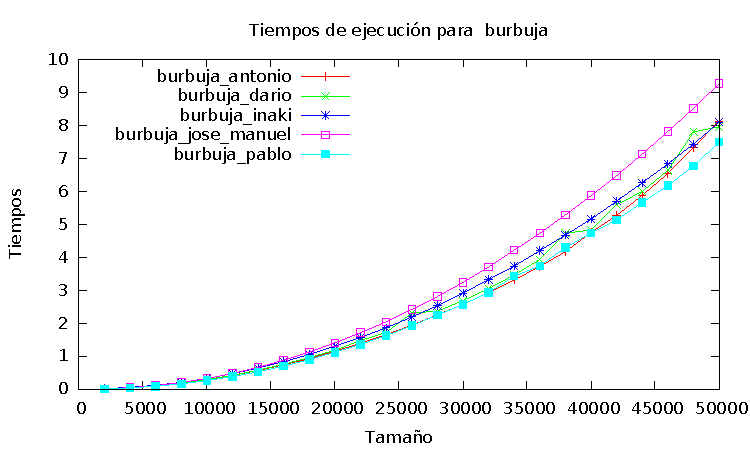
\includegraphics[width = \textwidth ]{burbuja_todos_g}
\end{frame}

\begin{frame}{Selección}
	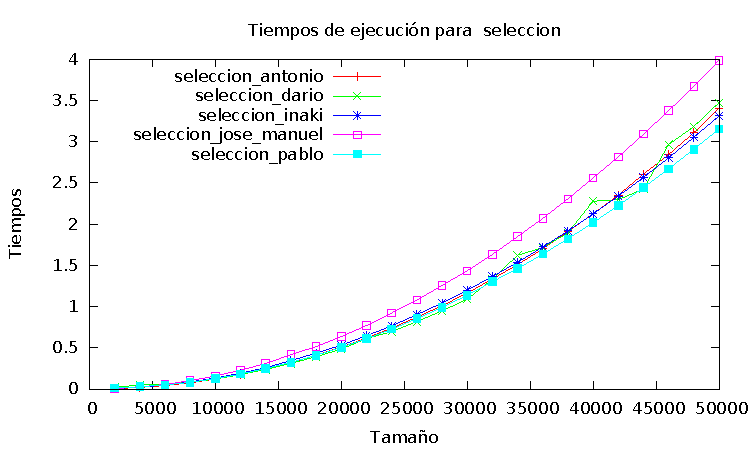
\includegraphics[width = \textwidth ]{seleccion_todos_g}
\end{frame}

\begin{frame}{Inserción}
	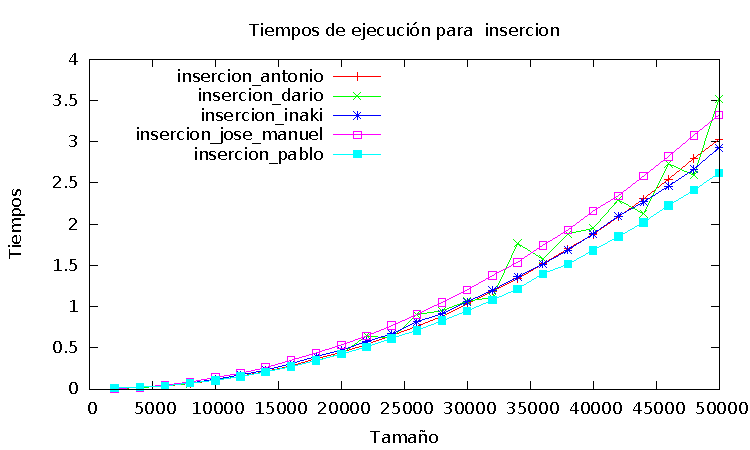
\includegraphics[width = \textwidth ]{insercion_todos_g}
\end{frame}

\begin{frame}{Comparativa: Algoritmos Cuadráticos}
	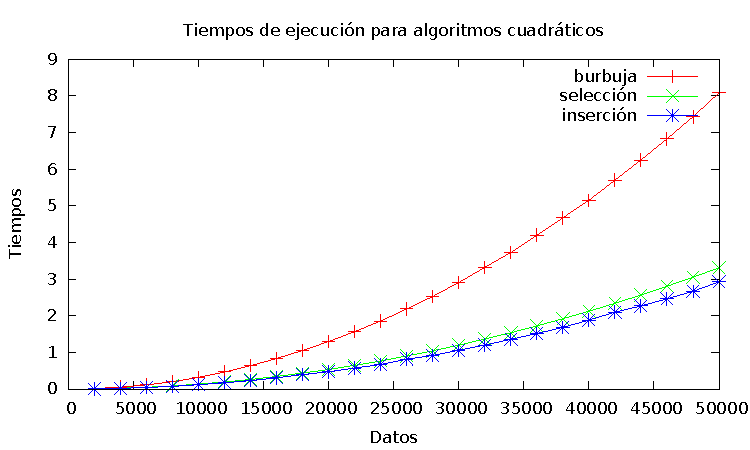
\includegraphics[width = \textwidth ]{comparativa_cuadraticos_g}
\end{frame}

\begin{frame}{Mergesort}
	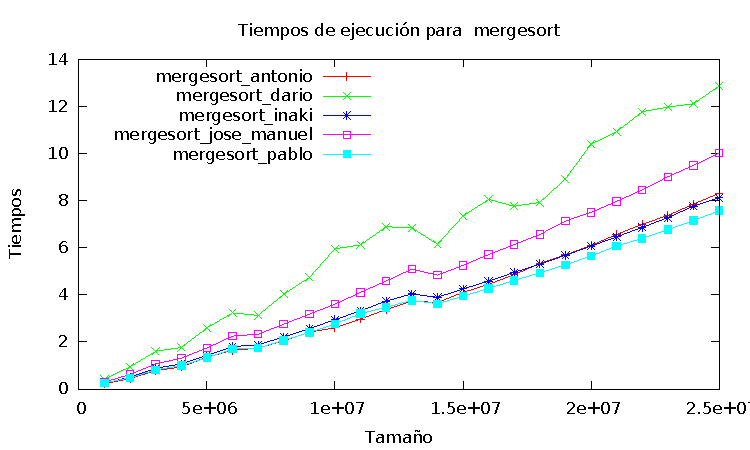
\includegraphics[width = \textwidth ]{mergesort_todos_g}
\end{frame}

\begin{frame}{Quicksort}
	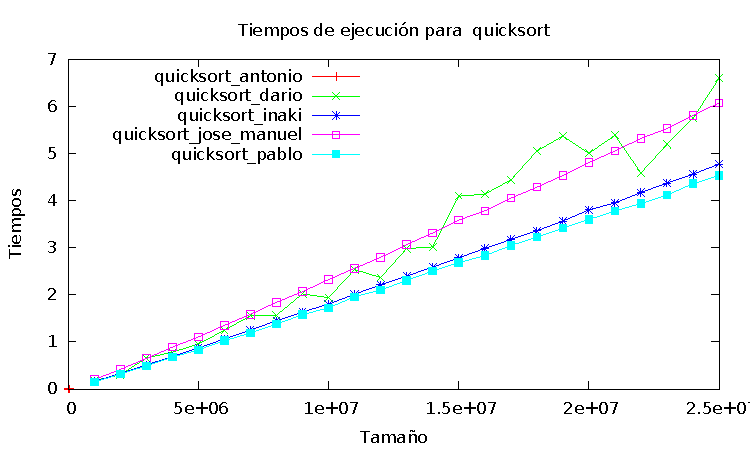
\includegraphics[width = \textwidth ]{quicksort_todos_g}
\end{frame}

\begin{frame}{Heapsort}
	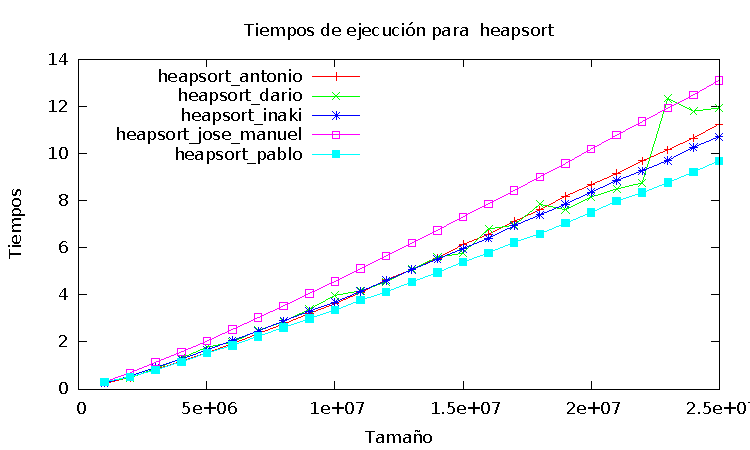
\includegraphics[width = \textwidth ]{heapsort_todos_g}
\end{frame}

\begin{frame}{Comparativa: Algoritmos O$(nlog(n))$}
		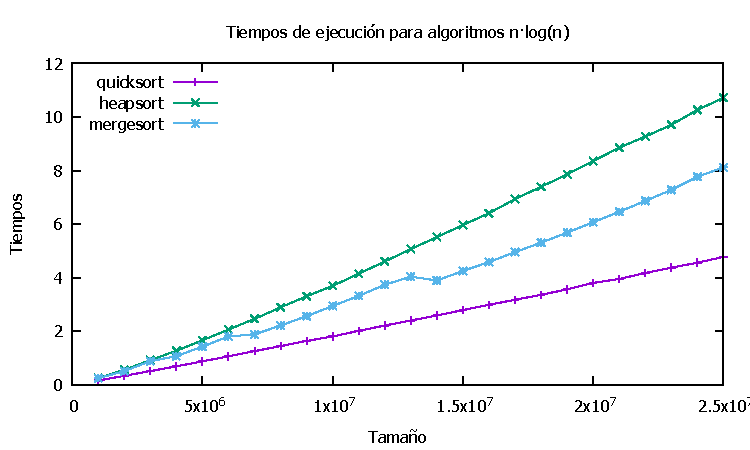
\includegraphics[width = \textwidth ]{comparativa_logaritmicos_g}
\end{frame}

\begin{frame}{Algoritmo de Floyd}
		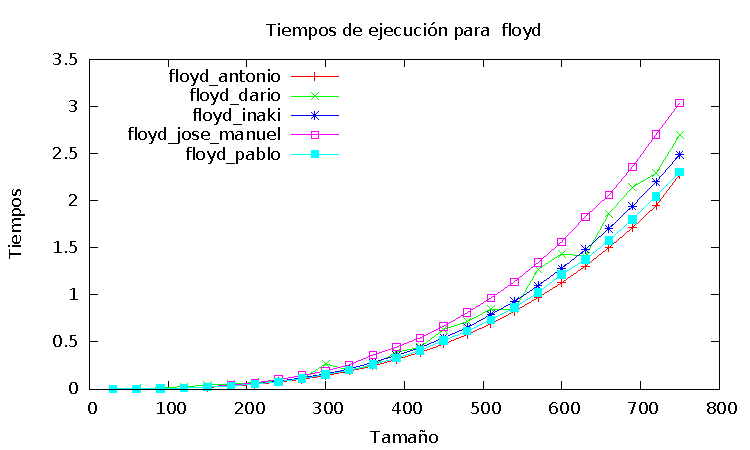
\includegraphics[width = \textwidth ]{floyd_todos_g}
\end{frame}

\begin{frame}{Fibonacci}
		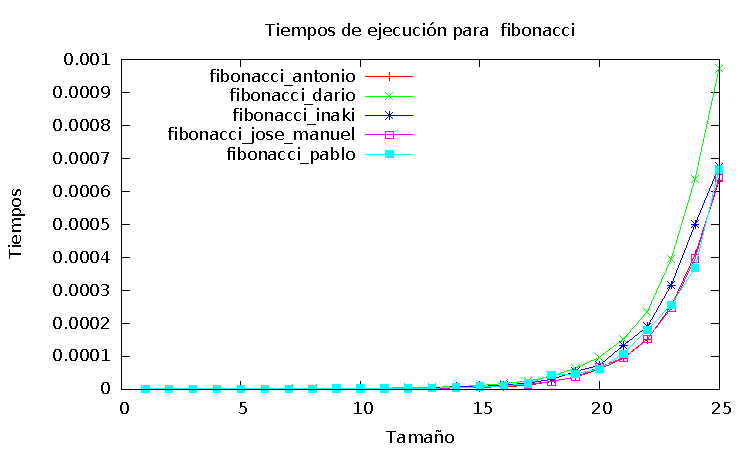
\includegraphics[width = \textwidth ]{fibonacci_todos_g}
\end{frame}

\begin{frame}{Hanói}
		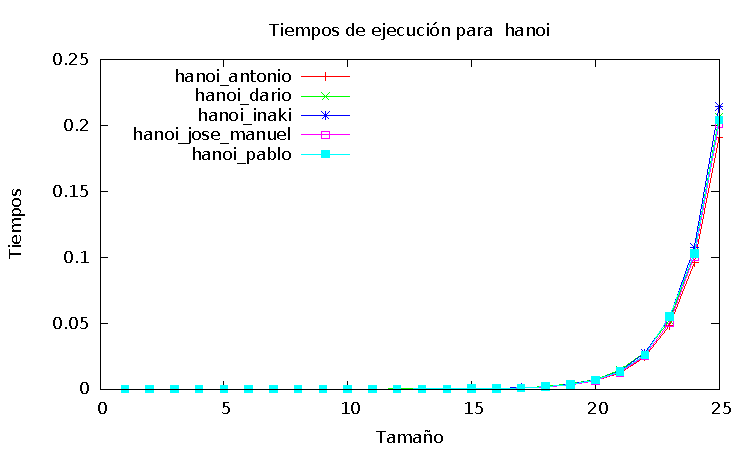
\includegraphics[width = \textwidth ]{hanoi_todos_g}
\end{frame}

\begin{frame}{Comparativa global de los algoritmos}
		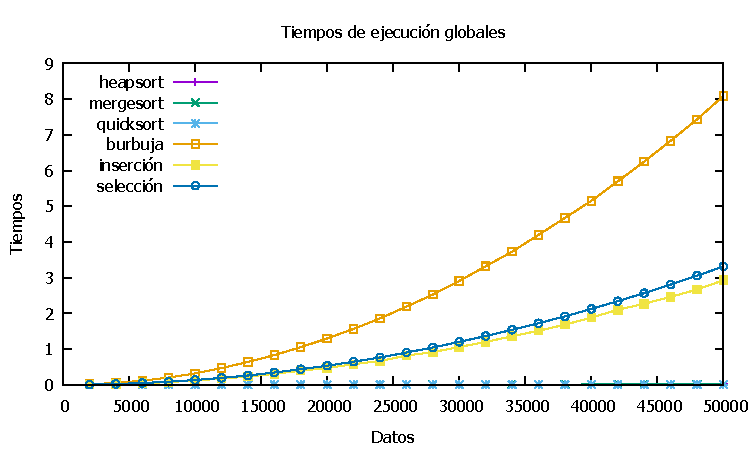
\includegraphics[width = \textwidth ]{comparativa_global_g}
\end{frame}


\section{Ejercicio 3: \large{Eficiencia Híbrida }}

\subsection{Parámetros de ajuste individuales}

\begin{frame}{Ajuste de Burbuja}
\noindent\adjustbox{max width=\textwidth}{%
\begin{tabular}{|l|l|}
	\hline
	Persona & Eficiencia híbrida de Burbuja \\
	\hline

	Antonio & $3.67\cdot 10^{-9}n^2 -3.02\cdot 10^{-5}n + 0.189$ ($0.99$) \\
	\hline
	Darío &$89\cdot10^{-3} -1.62\cdot10^{-5}\cdot n +3\cdot10^{-9}\cdot n^2$ $ (0.99)$ \\

	\hline
	José Manuel & $3.85\cdot 10^{-9}n^2 - 7.88\cdot 10^{-6}n + 0.013$ ($0.99$) \\
	\hline
	Pablo & $3\cdot 10^{-9}n^2 -6\cdot 10^{-6}n + 0,015$ ($0.99$) \\
	\hline
	Iñaki & $3.23\cdot 10^{-9}n^2 +1.36\cdot 10^{-7}n -2.52\cdot 10^{-5}$ ($0.99$)\\
	\hline
\end{tabular}
}
\end{frame}

\begin{frame}{Ajuste de Inserción}
\noindent\adjustbox{max width=\textwidth}{%
\begin{tabular}{|l|l|}
	\hline
	Persona & Eficiencia híbrida de Inserción \\
	\hline
	Antonio &  $1.21\cdot 10^{-9}n^2 -5.77\cdot 10^{-6}n + 0,003$ ($0.99$)  \\
	\hline
	Darío &$89 \cdot 10^{-3}+-1.62\cdot10^{-5} \cdot n +1.68\cdot 10^{-9}\cdot n^2$ $ (0.99)$ \\
	\hline
	José Manuel  & $1.32\cdot 10^{-9}n^2 + 4.95\cdot 10^{-7}n - 0.0024$ ($0.99$) \\
	\hline
	Pablo & $10^{-9}n^2 + 4\cdot 10^{-7}n + 0,002$ ($0.99$) \\
	\hline
	Iñaki & $1.18\cdot 10^{-9}n^2 +1.36 \cdot 10^{-7}n -2.5\cdot 10^{-5}$ ($0.99$)\\
	\hline
\end{tabular}
}
\end{frame}

\begin{frame}{Ajuste de Selección}
\noindent\adjustbox{max width=\textwidth}{%
\begin{tabular}{|l|l|}
	\hline
	Persona & Eficiencia híbrida de Selección \\
	\hline

	Antonio &  $1.459 \cdot 10^{-9}n^2 -5.7\cdot 10^{-6}n + 0,002$ ($1$) \\
	\hline
	Darío &$89\cdot 10^{-3}-1.616\cdot 10^{-5}\cdot n +1.59 \cdot 10^{-9} \cdot n^2$ $(0.99)$ \\

	\hline
	José Manuel & $1.59\cdot 10^{-9}n^2 + 2.93 \cdot 10^{-7} n - 0.0022$ $(0.99)$ \\
	\hline
	Pablo & $10^{-9}n^2 -2\cdot 10^{-7}n + 0,004$ ($1$) \\
	\hline
	Iñaki & $1.31\cdot 10^{-9}n^2 +5.81\cdot 10^{-7} -0.002$ ($0.99$)\\
	\hline
\end{tabular}
}
\end{frame}

\begin{frame}{Ajustes $n \cdot \log(n)$}

\noindent\adjustbox{max width=\textwidth}{
\begin{tabular}{|l|l|l|l|}
	\hline
	Persona & Heapsort & Mergesort & Quicksort \\
	\hline

	Antonio & $2.72 \cdot 10^{-8}n\log(n) -0.55$ ($0.999$)  & $1.918 \cdot 10^{-8} n \log(n) - 0.305 $ ($0.996$)& $1.06 \cdot 10^{-8}n\log(n) -0.083 $ ($0.999$)\\
	\hline
	Darío & $2.56\cdot 10^{-8} n\log(n) -0.005$ $(0.99) $&$3.03\cdot 10^{-8}n\log(x) -0.004$ $(0.99)$&$1.46\cdot 10^{-8}\cdot n\log(n) -0.005$ $(0.99)$ \\

	\hline
	José Manuel & $3.13\cdot 10^{-8}n\log(n) - 0.37$ ($0.99$) & $2.29 \cdot 10^{-8}n\log(n) - 0.08$ ($0.99$) & $1.42 \cdot 10^{-8}n\log(n) + 0.02$ ($0.99$)\\
	\hline
	Pablo & $1.8 \cdot 10^{-8}n\log(n) -1.9\cdot 10^{-7}$ ($0.995$)  & $2 \cdot 10^{-8} n \log(n) - 1.9\cdot 10^{-7}$ ($0.997$)& $1.3 \cdot 10^{-8}n\log(n) -1.9\cdot 10^{-7}$ ($0.999$)\\
	\hline
	Iñaki & $2.46\cdot 10^{-8}n\log(n) +1.36\cdot 10^{-7}$ ($0.99$)
	& $1.48\cdot 10^{-8}n\log(n) +1$ ($0.99$)
	& $1.12\cdot 10^{-8}n\log(n) +1.36\cdot 10^{-7}$ ($0.99$)\\
	\hline

\end{tabular}
}

\end{frame}

\begin{frame}{Ajuste de Floyd}
\noindent\adjustbox{max width=\textwidth}{
\begin{tabular}{|l|l|l|}
	\hline
	Persona & Eficiencia híbrida de Floyd & $r$ \\
	\hline
	Antonio & $ 6 \cdot 10^{-9}n^3 -7.9 \cdot 10^{-7}n^2 -2.17 \cdot 10^{-4}n +0.012$ & $0.999$ \\
	\hline
	Darío & $6.98\cdot 10^{-9} \cdot n^3 -7.66\cdot 10^{-7}\cdot n^2 +0.0002\cdot n -0.005$ & $0.999$ \\

	\hline
	José Manuel & $ 6.88 \cdot 10^{-9}n^3 + 2.89 \cdot 10^{-7}n^2 -4.44 \cdot 10^{-5}n +0.001$ & $0.999$ \\
	\hline
	Pablo & $ 5.1 \cdot 10^{-9}n^3 + 3.8 \cdot 10^{-7}n^2 -8.3 \cdot 10^{-5}n +0.005$ & $1$ \\
	\hline
	Iñaki & $5.76\cdot 10^{-9}n^3 +1.36\cdot 10^{-7}n^2 -2.52\cdot 10^{-5}n +0.002$ & $0.999$\\
	\hline

\end{tabular}
}

\end{frame}

\begin{frame}{Ajuste de Fibonacci}
\noindent\adjustbox{max width=\textwidth}{
\begin{tabular}{|l|l|l|}

	\hline
	Persona & Eficiencia híbrida de Fibonacci & $r$ \\
	\hline

	Antonio & $3.81 \cdot 10^{-9} \varphi^n +7.21\cdot 10^{-7}$ & $0.999$\\
	\hline
	Darío & $0.002\cdot\varphi^n -0.004$ &$0.999$\\

	\hline
	José Manuel & $3.81 \cdot 10^{-9} \varphi^n +9.68\cdot 10^{-7}$ & $0.999$\\
	\hline
	Pablo & $6.4 \cdot 10^{-9} \varphi^n -1.8\cdot 10^{-8}$ & $0.997$\\
	\hline
	Iñaki & $4.29\cdot 10^{-9} \varphi^n +5.6\cdot 10^{-6}$ & $0.995$\\
	\hline
\end{tabular}}

\end{frame}

\begin{frame}{Ajuste de Hanoi}
\noindent\adjustbox{max width=\textwidth}{
	\begin{tabular}{|l|l|l|}
		\hline
		Persona & Eficiencia híbrida de Hanoi & $r$ \\
		\hline

		Antonio & $5.69 \cdot 10^{-9} 2^n + 1.1 \cdot 10^{-4}$ & $1$\\
		\hline
		Darío & $6.38\cdot 10^{-9}\cdot 2^n -0.005$ & $0.984$\\
		\hline
		José Manuel & $6.00 \cdot 10^{-9} 2^n + 9.3 \cdot 10^{-6}$ & $0.999$\\
		\hline
		Pablo & $6.1 \cdot 10^{-9} 2^n + 1.1 \cdot 10^{-9}$ & $0.998$\\
		\hline
		Iñaki & $6.39 \cdot 10^{-9} 2^n +9.48 \cdot 10^{-13}$ & $0.999$\\
		\hline
	\end{tabular}}
\end{frame}

\subsection{Ajustes con varias funciones}

\begin{frame}{Cuadráticos: inserción}
	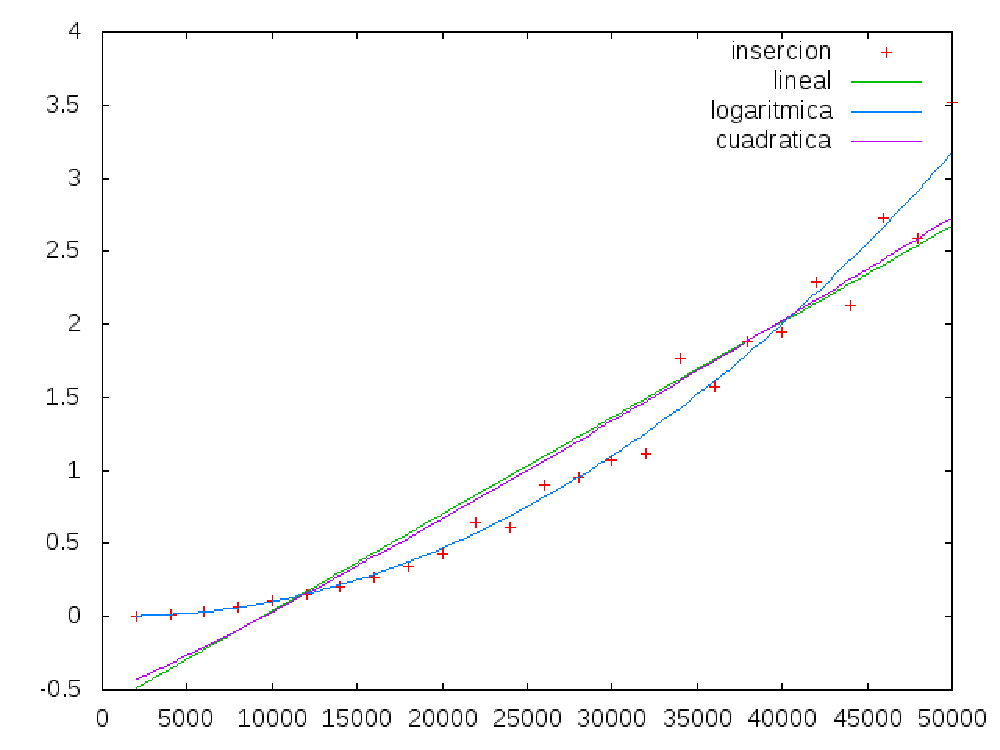
\includegraphics[width = \textwidth ]{img/cuad_hibrida.pdf}
\end{frame}

\begin{frame}{$n \cdot \log(n)$: quicksort}
	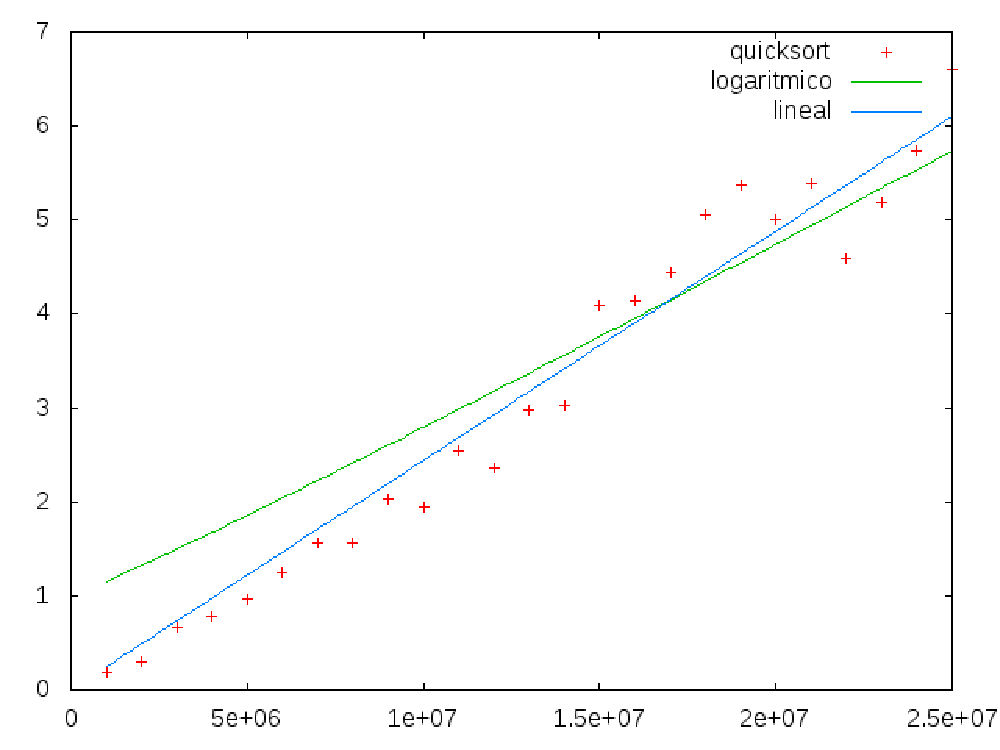
\includegraphics[width = \textwidth ]{img/log_hibrida.pdf}
\end{frame}

\begin{frame}{Exponenciales: Hanoi}
	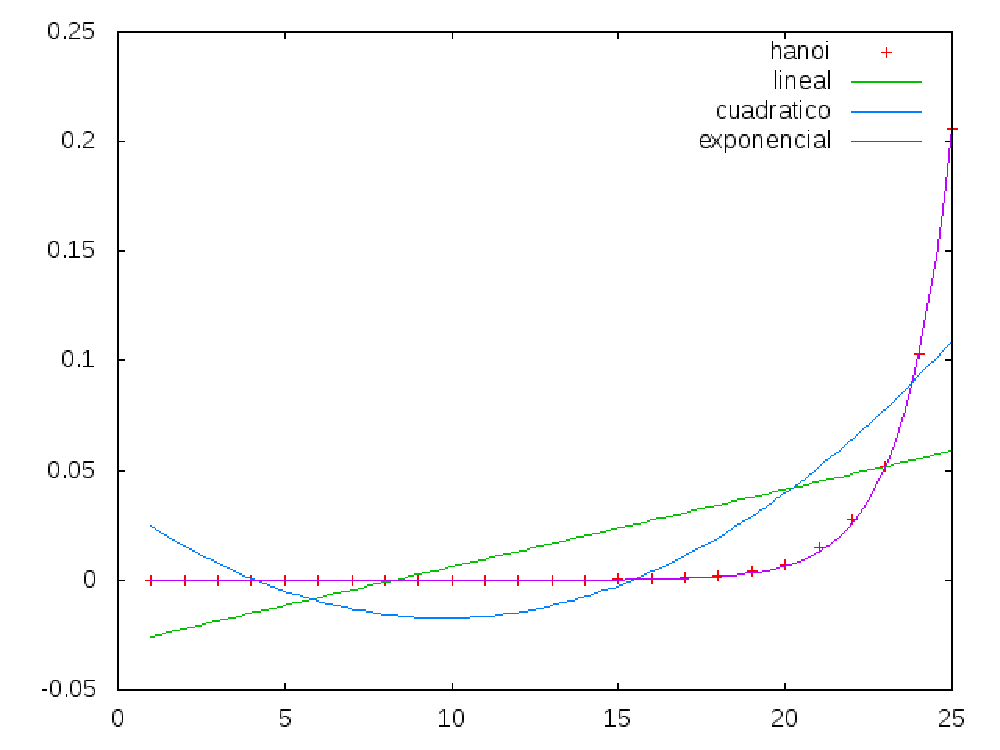
\includegraphics[width = \textwidth ]{img/expo_hibrida2.pdf}
\end{frame}

\begin{frame}{Cúbicos: Floyd}
	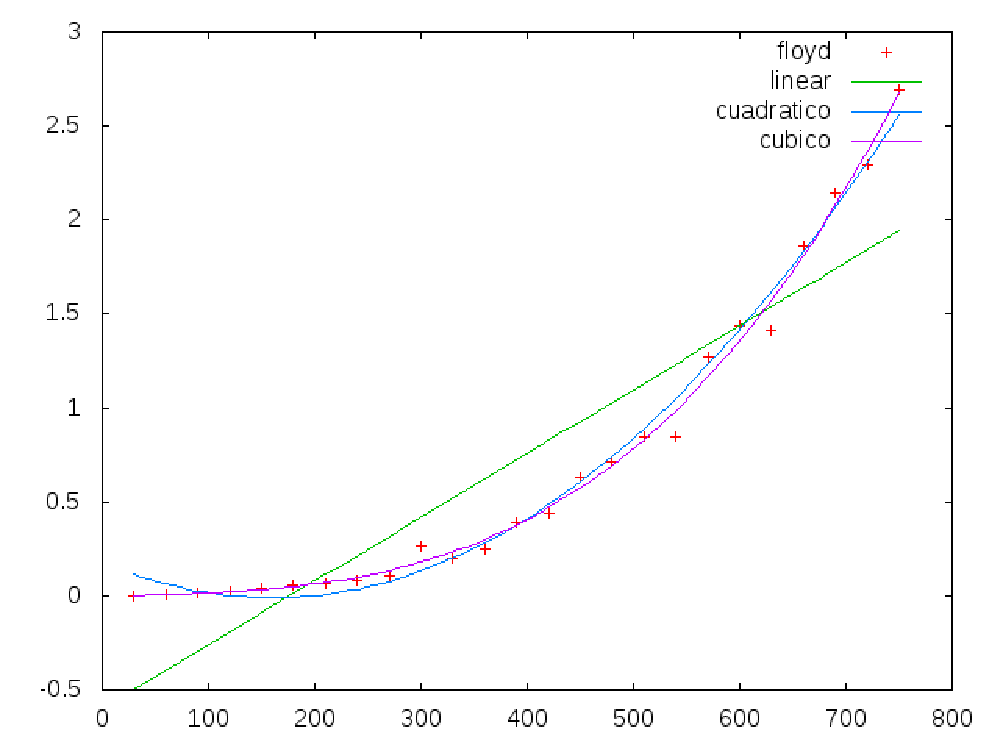
\includegraphics[width = \textwidth ]{img/floyd_hibrida.pdf}
\end{frame}

\section{Ejercicio 4: \large{Eficiencia según la optimización }}

\subsection{Algoritmos cuadráticos}

\begin{frame}{Burbuja}
	\begin{tabular}{|l|l|l|l|l|}
	\hline
	Tamaño & O0 & O1 & O2 & O3 \\
	\hline
	\hline
	2000 & 0,011413 & 0,00767027 & 0,00729825 & 0,00886811 \\
	\hline
	10000 & 0,285049 & 0,124228 & 0,109425 & 0,10953 \\
	\hline
	18000 & 0,9231 & 0,450813 & 0,402396 & 0,400231 \\
	\hline
	26000 & 1,93603 & 0,983933 & 0,869556 & 0,865144 \\
	\hline
	34000 & 3,31074 & 1,74399 & 1,51139 & 1,51782 \\
	\hline
	42000 & 5,26566 & 2,70633 & 2,3327 & 2,40839 \\
	\hline
	50000 & 8,1269 & 3,92439 & 3,36591 & 3,64032 \\
	\hline
\end{tabular}

\end{frame}

\begin{frame}{Burbuja}
	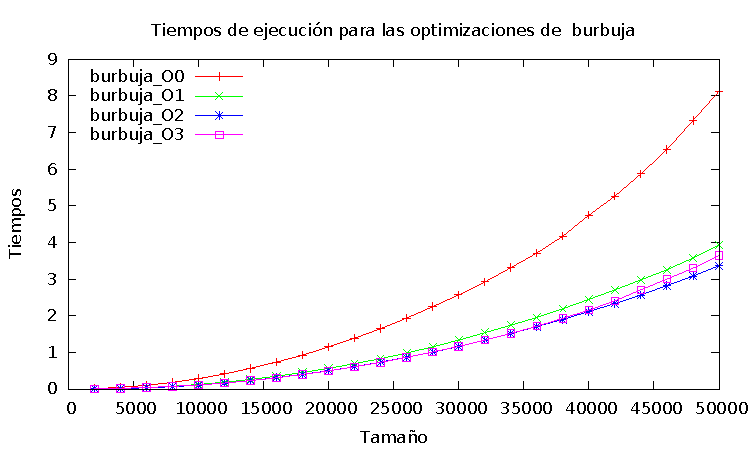
\includegraphics[width = \textwidth ]{img/burbuja_optim_g.pdf}
\end{frame}

\begin{frame}{Selección}
	\begin{tabular}{|l|l|l|l|l|}
	\hline
	Tamaño & O0 & O1 & O2 & O3 \\
	\hline
	\hline
	2000 & 0,00515467 & 0,00518568 & 0,00295874 & 0,00781173 \\
	\hline
	10000 & 0,121217 & 0,0446664 & 0,0325282 & 0,0535996 \\
	\hline
	18000 & 0,410265 & 0,0952006 & 0,0954893 & 0,162643 \\
	\hline
	26000 & 0,872412 & 0,202472 & 0,197149 & 0,347695 \\
	\hline
	34000 & 1,50895 & 0,347973 & 0,335636 & 0,602817 \\
	\hline
	42000 & 2,35229 & 0,538412 & 0,513721 & 0,930382 \\
	\hline
	50000 & 3,40647 & 0,766349 & 0,725693 & 1,3503 \\
	\hline
\end{tabular}

\end{frame}

\begin{frame}{Selección}
	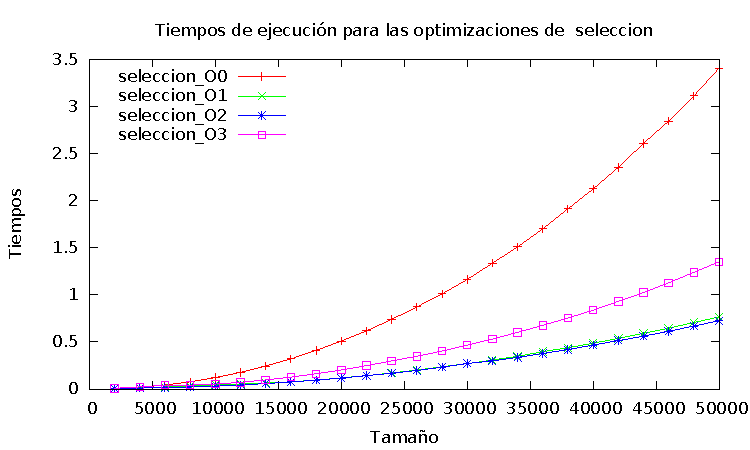
\includegraphics[width = \textwidth ]{img/seleccion_optim_g.pdf}
\end{frame}

\begin{frame}{Inserción}
	\begin{tabular}{|l|l|l|l|l|}
	\hline
	Tamaño & O0 & O1 & O2 & O3 \\
	\hline
	\hline
	2000 & 0,0044917 & 0,00195844 & 0,00468466 & 0,00632375 \\
	\hline
	10000 & 0,107932 & 0,037316 & 0,0457049 & 0,0458144 \\
	\hline
	18000 & 0,368311 & 0,120639 & 0,138311 & 0,137761 \\
	\hline
	26000 & 0,760331 & 0,257764 & 0,301838 & 0,295198 \\
	\hline
	34000 & 1,33726 & 0,444824 & 0,492365 & 0,497819 \\
	\hline
	42000 & 2,08887 & 0,679748 & 0,747116 & 0,773843 \\
	\hline
	50000 & 3,02904 & 0,987499 & 1,05693 & 1,11367 \\
	\hline
\end{tabular}

\end{frame}

\begin{frame}{Inserción}
	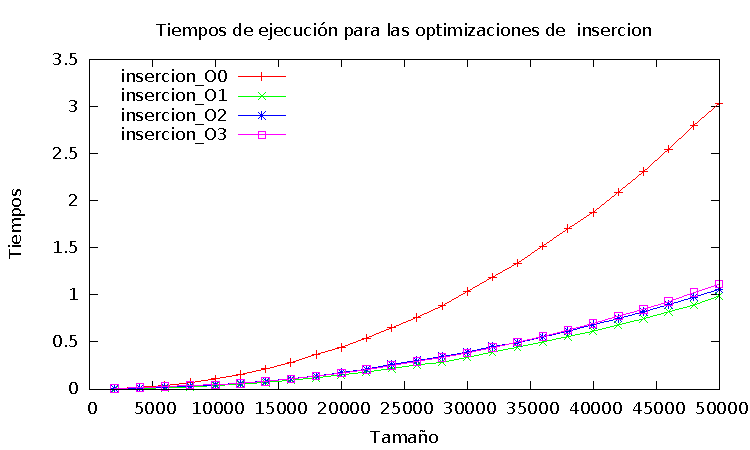
\includegraphics[width = \textwidth ]{img/insercion_optim_g.pdf}
\end{frame}

\subsection{Algoritmos $n \cdot \log(n)$}

\begin{frame}{Quicksort}
	\begin{tabular}{|l|l|l|l|l|}
	\hline
	Tamaño & O0 & O1 & O2 & O3 \\
	\hline
	\hline
	1000000 & 0,140354 & 0,108984 & 0,0723194 & 0,145934 \\
	\hline
	5000000 & 0,768809 & 0,4443 & 0,444097 & 0,413716 \\
	\hline
	9000000 & 1,43536 & 0,744798 & 0,842272 & 0,768711 \\
	\hline
	13000000 & 2,12925 & 1,11231 & 1,2527 & 1,15554 \\
	\hline
	17000000 & 2,81701 & 1,70221 & 1,69107 & 1,52156 \\
	\hline
	21000000 & 3,69781 & 2,17781 & 2,11261 & 1,8951 \\
	\hline
	25000000 & 4,59738 & 2,68214 & 2,59766 & 2,34848 \\
	\hline
\end{tabular}

\end{frame}

\begin{frame}{Quicksort}
	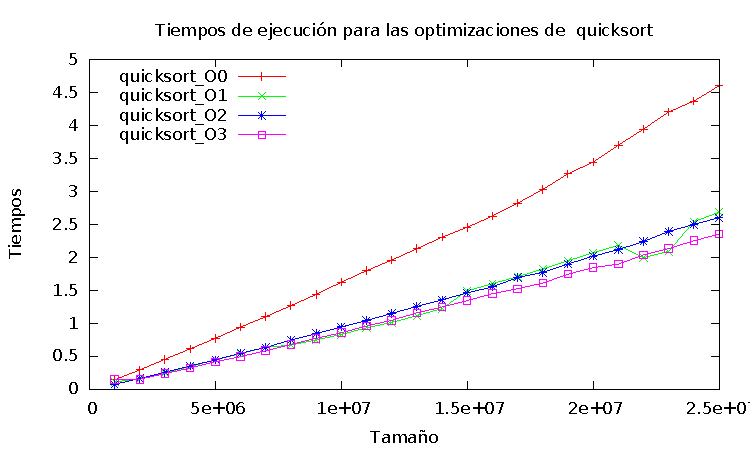
\includegraphics[width = \textwidth ]{img/quicksort_optim_g.pdf}
\end{frame}

\begin{frame}{Mergesort}
	\begin{tabular}{|l|l|l|l|l|}
	\hline
	Tamano & O0 & O1 & O2 & O3 \\
	\hline
	\hline
	1000000 & 0,217543 & 0,14913 & 0,155871 & 0,142481 \\
	\hline
	5000000 & 1,35111 & 0,605842 & 0,626561 & 0,673165 \\
	\hline
	9000000 & 2,41358 & 1,12709 & 1,15498 & 1,21198 \\
	\hline
	13000000 & 3,73061 & 1,76984 & 1,86878 & 1,66805 \\
	\hline
	17000000 & 4,85593 & 2,28211 & 2,35156 & 2,44318 \\
	\hline
	21000000 & 6,56725 & 3,00782 & 3,05882 & 2,74309 \\
	\hline
	25000000 & 8,30719 & 3,76735 & 3,90997 & 4,03064 \\
	\hline
\end{tabular}

\end{frame}

\begin{frame}{Mergesort}
	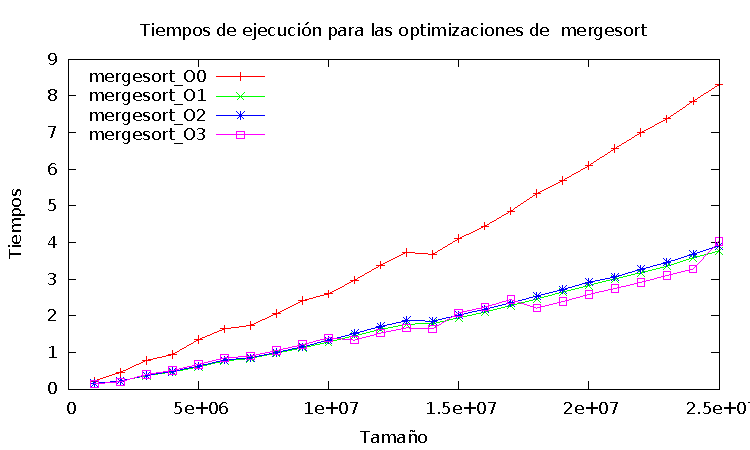
\includegraphics[width = \textwidth ]{img/mergesort_optim_g.pdf}
\end{frame}

\begin{frame}{Heapsort}
	\begin{tabular}{|l|l|l|l|l|}
	\hline
	Tamano & O0 & O1 & O2 & O3 \\
	\hline
	\hline
	1000000 & 0,22421 & 0,162612 & 0,189088 & 0,124874 \\
	\hline
	5000000 & 1,54404 & 0,996273 & 0,776043 & 0,797603 \\
	\hline
	9000000 & 3,20945 & 2,41538 & 1,59403 & 1,65914 \\
	\hline
	13000000 & 5,0709 & 4,02955 & 2,52116 & 2,54731 \\
	\hline
	17000000 & 7,11513 & 5,97832 & 3,9232 & 3,5468 \\
	\hline
	21000000 & 9,14739 & 7,9527 & 4,99053 & 4,66293 \\
	\hline
	25000000 & 11,2477 & 9,74256 & 6,22192 & 5,78521 \\
	\hline
\end{tabular}

\end{frame}

\begin{frame}{Heapsort}
	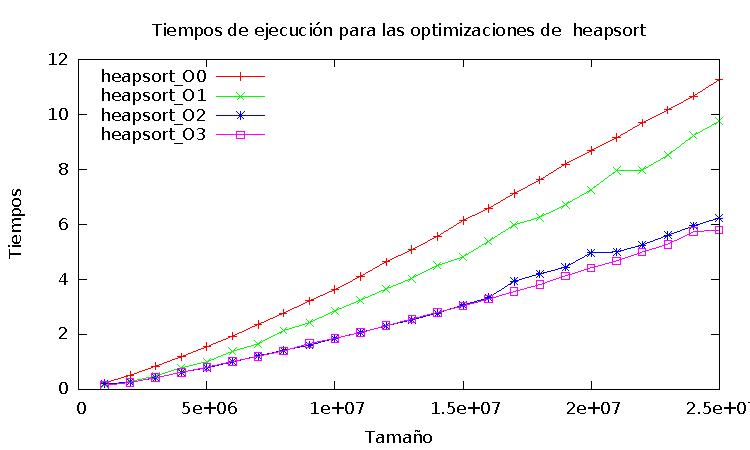
\includegraphics[width = \textwidth ]{img/heapsort_optim_g.pdf}
\end{frame}

\subsection{Algoritmos cúbicos}

\begin{frame}{Floyd}
	\begin{tabular}{|l|l|l|l|l|}
	\hline
	Tamaño & O0 & O1 & O2 & O3 \\
	\hline
	\hline
	30 & 0,000224592 & 0,00011651 & 5,3519e-05 & 8,2696e-05 \\
	\hline
	150 & 0,0186866 & 0,00662406 & 0,00634183 & 0,00455262 \\
	\hline
	270 & 0,104221 & 0,029449 & 0,0166624 & 0,0174797 \\
	\hline
	390 & 0,314773 & 0,0663636 & 0,052403 & 0,0504283 \\
	\hline
	510 & 0,692464 & 0,14376 & 0,114807 & 0,115598 \\
	\hline
	630 & 1,30571 & 0,269596 & 0,207239 & 0,227301 \\
	\hline
	750 & 2,27876 & 0,456356 & 0,349434 & 0,374203 \\
	\hline
\end{tabular}

\end{frame}

\begin{frame}{Floyd}
	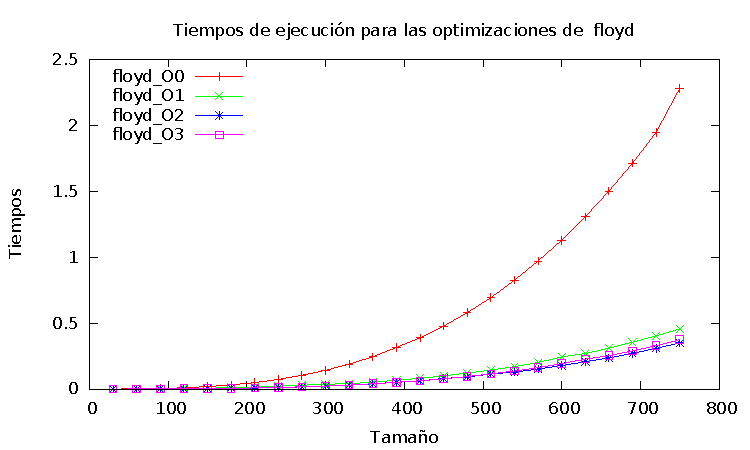
\includegraphics[width = \textwidth ]{img/floyd_optim_g.pdf}
\end{frame}

\subsection{Algoritmos exponenciales}

\begin{frame}{Fibonacci}
	\begin{tabular}{|l|l|l|l|l|}
	\hline
	Tamaño & O0 & O1 & O2 & O3 \\
	\hline
	\hline
	1 & 1,44e-07 & 3,74e-07 & 4,1e-07 & 4,05e-07 \\
	\hline
	5 & 3,51e-07 & 6,09e-07 & 4,66e-07 & 3,84e-07 \\
	\hline
	9 & 8,29e-07 & 1,177e-06 & 9,62e-07 & 7,74e-07 \\
	\hline
	13 & 2,937e-06 & 3,159e-06 & 2,467e-06 & 2,21e-06 \\
	\hline
	17 & 1,1107e-05 & 1,4243e-05 & 1,1615e-05 & 8,258e-06 \\
	\hline
	21 & 9,3336e-05 & 9,188e-05 & 7,0517e-05 & 4,4614e-05 \\
	\hline
	25 & 0,000630981 & 0,000592224 & 0,000359381 & 0,000286624 \\
	\hline
\end{tabular}

\end{frame}

\begin{frame}{Fibonacci}
	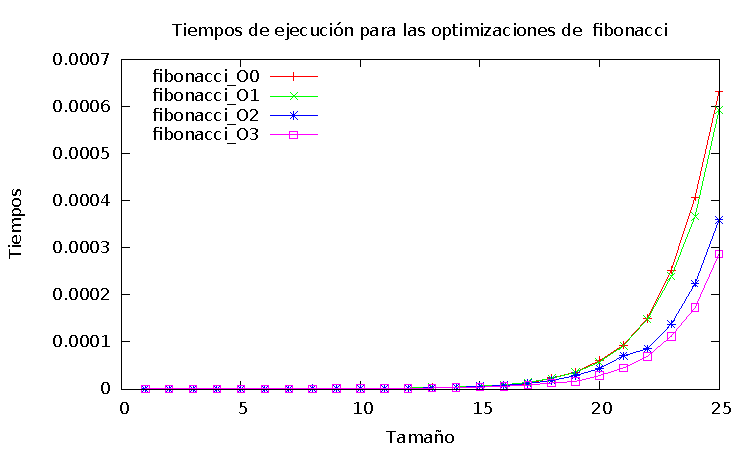
\includegraphics[width = \textwidth ]{img/fibonacci_optim_g.pdf}
\end{frame}

\begin{frame}{Hanói}
	\begin{tabular}{|l|l|l|l|l|}
	\hline
	Tamaño & O0 & O1 & O2 & O3 \\
	\hline
	\hline
	1 & 1,79e-07 & 2,03e-07 & 3,96e-07 & 3,6e-07 \\
	\hline
	5 & 6,54e-07 & 4,43e-07 & 1,256e-06 & 6,19e-07 \\
	\hline
	9 & 4,721e-06 & 2,48e-06 & 4,946e-06 & 3,05e-06 \\
	\hline
	13 & 6,5735e-05 & 2,4637e-05 & 5,0217e-05 & 2,3284e-05 \\
	\hline
	17 & 0,000772841 & 0,000387059 & 0,000577299 & 0,000286237 \\
	\hline
	21 & 0,0121097 & 0,00643389 & 0,00811653 & 0,00335663 \\
	\hline
	25 & 0,19084 & 0,0969232 & 0,0829641 & 0,0535821 \\
	\hline
\end{tabular}

\end{frame}

\begin{frame}{Hanói}
	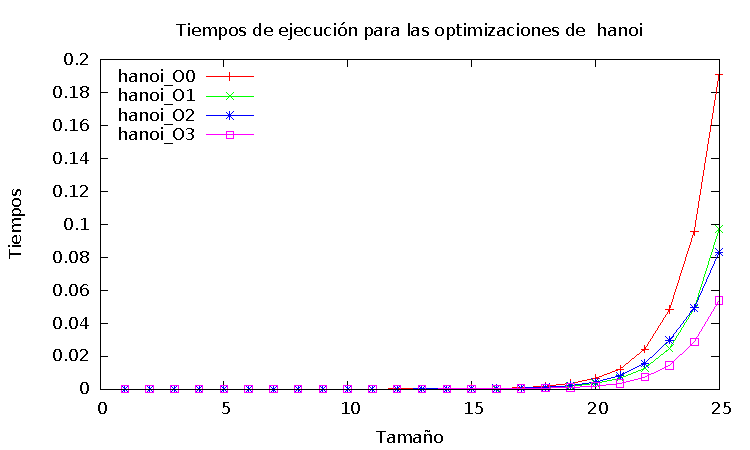
\includegraphics[width = \textwidth ]{img/hanoi_optim_g.pdf}
\end{frame}

\end{document}
